In this section we present the results we came up during the tests altogether with the conclusions, in order to provide a better overview of the tests that have been performed. 

\subsection{Comparison against dgemm}

Against the $dgemm()$ library function, even with the same compiling options, the implementation provided of the $matmult\_nat()$ method has been proven poor, according to the graph shown in Figure \ref{fig:natdgemmcomp}. The figure shown that, for every possible permutation of the cycle order (including so the naive implementation), dgemm outnumbers it.

\begin{figure}[here]
\centering
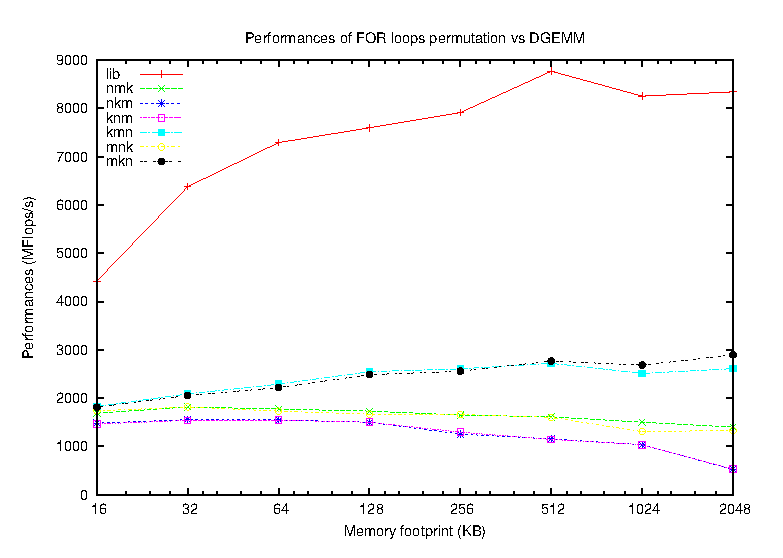
\includegraphics[width=\textwidth]{results/dgemm.eps}
\caption{Comparison between \emph{dgemm()} and the other implementations.}
\label{fig:natdgemmcomp}
\end{figure}

The reason for that is that the $dgemm()$ library has been a lot of years in the industry, and has received a lot of performance improvements during the years. In addition, the library makes use of some inline assembly codes that boost its performance even more.

\subsection{Permutations of m, k, n and performance}
The three cycles performed in the naive algorithm can be rearrenged in six different ways: there are in fact six possible permutations of the three letters. The performance results provided by the execution of the six algorithms on some standards memory footprints are provided in Figure \ref{fig:permutations}. The test was made on the product of square matrices $nxnxn$, where $n$ was calculated using the following formula, to relate it to the memory footprint:

\begin{figure}[here]
\centering
\includegraphics[width=\textwidth]{results/permutations.eps}
\caption{The possible combinations of \emph{matmult\_xxx()} for the Intel processor on square matrices of growing size.}
\label{fig:permutations}
\end{figure}

$$
n = \sqrt{\frac{F_{byte}}{8 \cdot 3} }
$$

The best results of the graph are the ones where the most internal cycle is cycled over $[1,n]$, and in particular the best implementation has been proved $m-k-n$, followed by $k-m-n$. The worst ones, instead, have been proved $n-k-m$ and $k-n-m$, the ones with the most internal cycle in m.

The result was what we expected in the Theory section. As a recall, the explanation of this behaviour is that $m-k-n$ is the best implementation because is the one that causes the less cache misses. If the most internal variable looped is $n$, in fact, we read a whole row in the matrix each time we start reading an element from matrices $B$ and $C$ (that have both $n$ columns). This causes less misses in the cache, leading to a better perfomance for both the $m-k-n$ and $k-m-n$ behaviours. In addition, since the A matrix has k columns, also if we loop through k before looping though m we got a better performance, for the same reason. This explains why $m-k-n$ is slighly better that  the $k-m-n$ implementation.

The worst case scenarios  $n-k-m$ and $k-n-m$, instead, do the opposite: they privilegiate columns over rows, resulting in a better performance if the matrix was stored column-wise, like in Fortran, but leading to disastruous results in C, where the most performant is the rowmajor order.

To verificate our assumption, we checked the number of cache misses for both the best and the worst implementation, resulting in:

\vspace{10pt} 
\begin{tabular}{ l l l}
\hline
 & knm& mkn\\ \hline
MFlops:        &  440.342& 1548.554 \\ \hline
Misses in L1-Data:     & 3 969 996 464 & 2 239 998 044 \\ \hline
Misses in L2-Data:     & 99 000 394 & 102 000 309\\ \hline

\end{tabular}

\vspace{10pt} 

That confirmed our assumptions, seeing that the best implementation has fewer cache misses that the worst one.

\subsection{Performance of n,k,m implementations with different sizes}
The results and conclusions presented in the previous section held keeping in mind that the matrices we tested were square ones, where $n=m=k$. We repeated the same tests for some odd-sized matrices, i.e. where one of the three dimensions $n$,$m$,$k$ was kept at a low value (in these tests 4 elements). The other two values were raised accordingly, in order to maintain the same memory footprint and have meaningful results. The results we came up for n and am were pretty much the same, but we k we found some different results, which are presented on Figure \ref{fig:lowk}.

\begin{figure}[here]
\centering
\includegraphics[width=\textwidth]{results/littlek.eps}
\caption{The possible combinations of \emph{matmult\_xxx()} with AMD processor.}
\label{fig:lowk}
\end{figure}

We can see that the performances of the two best version in the square case are dropped dramatically, especially for little memory footprints. Since the test is on the AMD processor, we are able do see a drop in the performance due to the filling up of the L1 cache around $128kB$ (the cache is actually 64K, but it seems a little larger due to prefetch). For matrix sizes, we can see that the results of the cache analysis still confirm our previous assumptions of $m-k-n$ being faster than $knm$, as shown in the following table:


\vspace{10pt} 
\begin{tabular}{ l l l}
\hline
 & knm& mkn\\ \hline
MFlops:        &  474.607& 741.996 \\ \hline
Misses in L1-Data:     & 2 419 072 580 & 6 600 200 \\ \hline
Misses in L2-Data:     & 272 000 807 & 164 000 494\\ \hline

\end{tabular}

\vspace{10pt} 

As a side note, even the $dgemm()$ library drops its performances roughly from 8GFlops to 2 GFlops, as it is optimized for square memory sizes.

\clearpage
\subsection{Blocked Matrix performance}
We recall that the blocked version, introduced in section Implementation, uses the best algorithm for naive multiplication, $m-k-n$, in its inner loop. We experimented the block size against the MFLOPs generated for a generally big square matrix (with $2048kB$ memory footprint). The results are reported in Figure \ref{lowk} (green line). The performances of the algorithm increased at the rising of the block size. This means that the optimum is the highest possible value of the block size, i.e. the matrix itself. In conclusion, the blocking algorithm can not really improve performance, because it will be always beaten by the $m-k-n$ algorithm. 

\begin{figure}[here]
\centering
\includegraphics[width=\textwidth]{results/blkwrong.eps}
\caption{The possible combinations of \emph{matmult\_xxx()} with AMD processor.}
\label{fig:lowk}
\end{figure}

To find an approximate optimum for the block size, it was necessary to substitute the algorithm in the inner loop with the worst one ($k-n-m$). Repeating the test, the data showed a plateau curve, reaching its maximum in the range 27-37. After 40, the performances start to decrease, because the L1d cache starts to fill up. At 40, in fact, we have an estimated data cache size of $3 \cdot 40^2 \cdot 8 = 37.5kB$, which is sligthly higher than the L1-data cache size ($32kB$) due to the prefetching effect.  

\begin{figure}[here]
\centering
\includegraphics[width=\textwidth]{results/3way.eps}
\caption{Comparison between $dgemm()$, the best blocked version and the $m-k-n$ Implementation.}
\label{fig:3way}
\end{figure}
\clearpage
\section{Compiler Options}
The compiler options tested where:
\begin{itemize}
\item \textbf{none} No optimization
\item \textbf{-xO1 to -xO5} Different levels of optimization. The higher the number the more aggressively the compiler tries to optimiz the code for performance.
\item \textbf{-xrestrict} Treats pointer-valued function parameters as restricted pointers. A restricted pointers are assumed not to be aliased. This flag improves vectorization.
\item \textbf{-fast} Macro that applies various options including -xO5. 
\end{itemize}
The different options was tested for different memory footprints on both an the AMD and Intel CPU. The results are given on figure \ref{fig:compilerOptionsAmd} and \ref{fig:compilerOptionsIntel}.
\begin{figure}[here]
\centering
\includegraphics[width=0.8\textwidth]{results/flag-test-plot-intel.eps}
\caption{Timings of different compiler options on the intel CPU}
\label{fig:compilerOptionsIntel}
\end{figure}
\begin{figure}[here]
\centering
\includegraphics[width=0.8\textwidth]{results/flag-test-plot-amd.eps}
\caption{Timings of different compiler options on the AMD CPU}
\label{fig:compilerOptionsAmd}
\end{figure}
\\\\
The fastest set of options on both the AMD and Intel is -fast -xO3 -xrestrict. The missing data points on figure \ref{fig:compilerOptionsAmd} is because test failed because of a compiler error whenever -fast. 
\\\\
As it can be seen from figure \ref{fig:3way} and figure \ref{fig:compilerOptionsIntel} that even though we use the fastest options we cannot compile a version of our implementation that is faster than the library function. 
\\\\
It is also interesting to note that options -x04 and -x05 performs worse than -xO3 on both the Intel and AMD. 

